\chapter{results}\label{results}


\section{ghsep}\label{ghsep}

The random forest for the gamma-/hadron-separation gets trained on 
XXX diffuse gamma events and XXX diffuse proton events with a 5-fold cross-validation.
With this, the model reaches an AUC 
of XXXX on the cross-validated set of diffuse gammas, as can be seen in figure \ref{fig:gh_roc}.

\begin{figure}
    \centering
    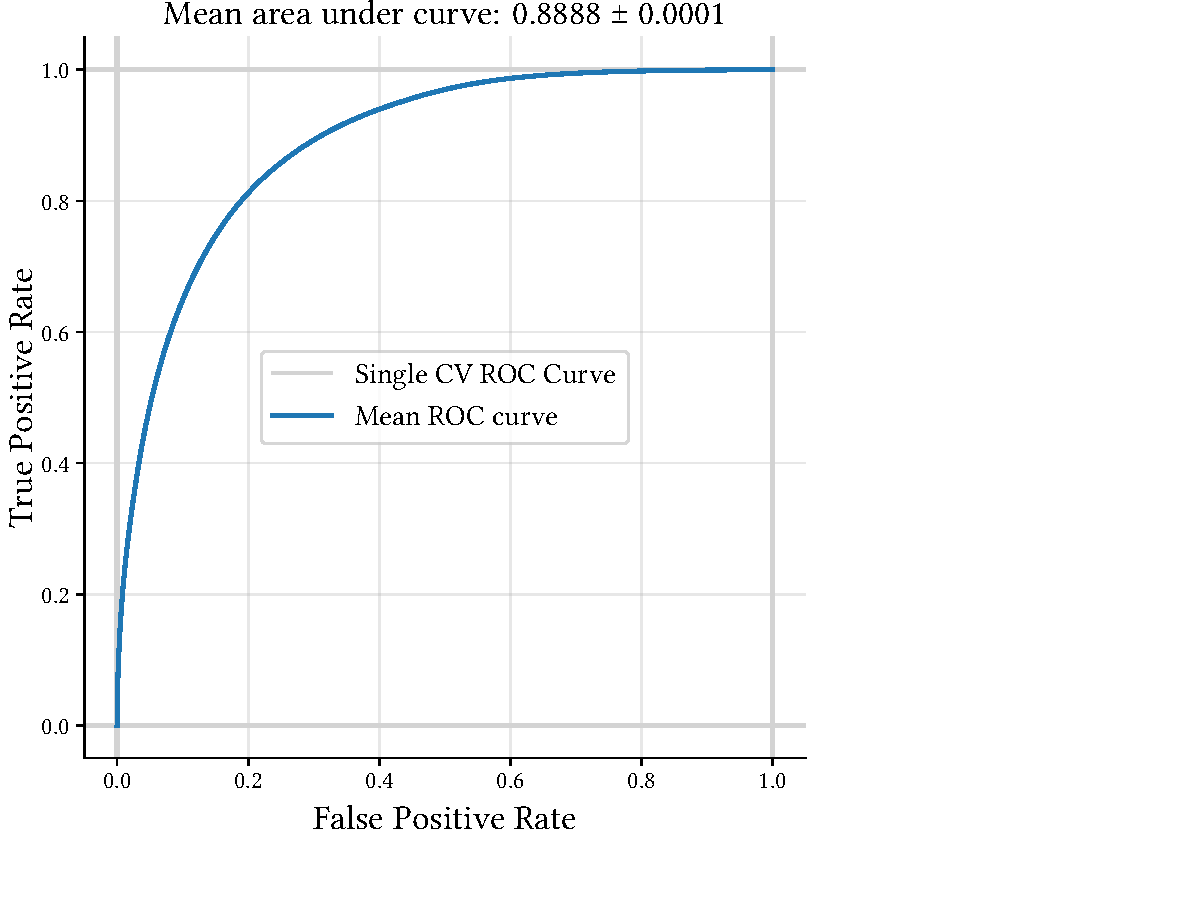
\includegraphics[page=1, width=.8\textwidth]{../analysis/plots/cross_val_sep_perf_plot.pdf}
    \caption{ROC for the gamma/hadron separation on the cross validated training set 
    consisting of XXX proton events and YYY diffuse gamma events (make dummy column on the left to center properly?).}
    \label{fig:gh_roc}
\end{figure}

The feature importance, as defined in chapter XXX, is shown in \ref{fig:gh_features}.
\begin{figure}
    \centering
    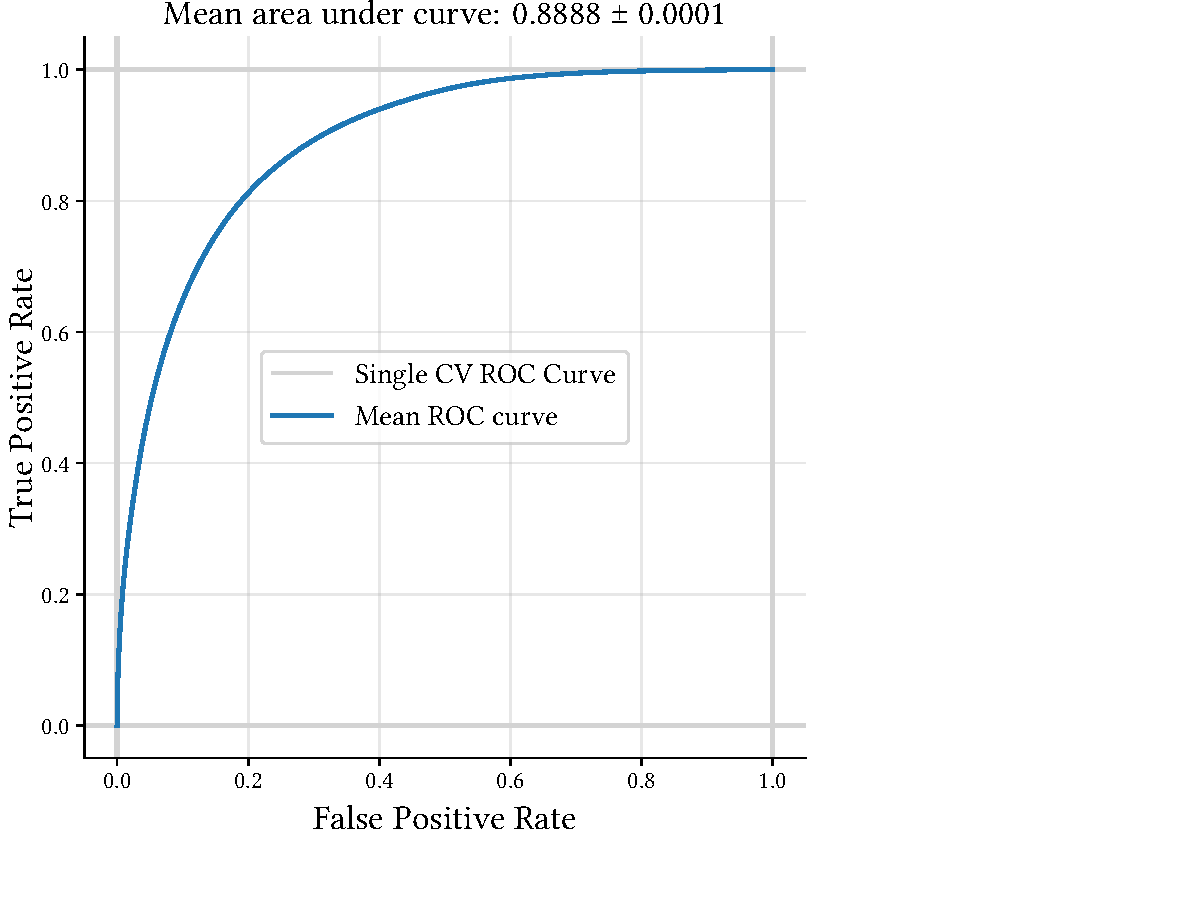
\includegraphics[page=1, width=.8\textwidth]{../analysis/plots/cross_val_sep_perf_plot.pdf}
    \caption{Feature importance for the gamma/hadron separation. Need to get that plot form the model!}
    \label{fig:gh_features}
\end{figure}


From our XXXX pointlike gamma events that we test our reconstruction method on, 
XXX \% get the correct label.
